\chapter{Сравнение}

\section{Сравнение эмпирических и аналитических результатов}
Для того, чтобы убедиться в правильности построения и анализа модели, проведём сравнение результатов, полученных эмпирическим и теоретическим способами.
Для этого произведем симуляцию на языке Python 3 и сравним полученные результаты с результатами теоретическими.
Помимо самого языка, для симуляции поведения модели использовалась библиотека для работы с графами networkx.
В данном случае использовано $200$ симулированных процессов.

\begin{figure}[h!]
    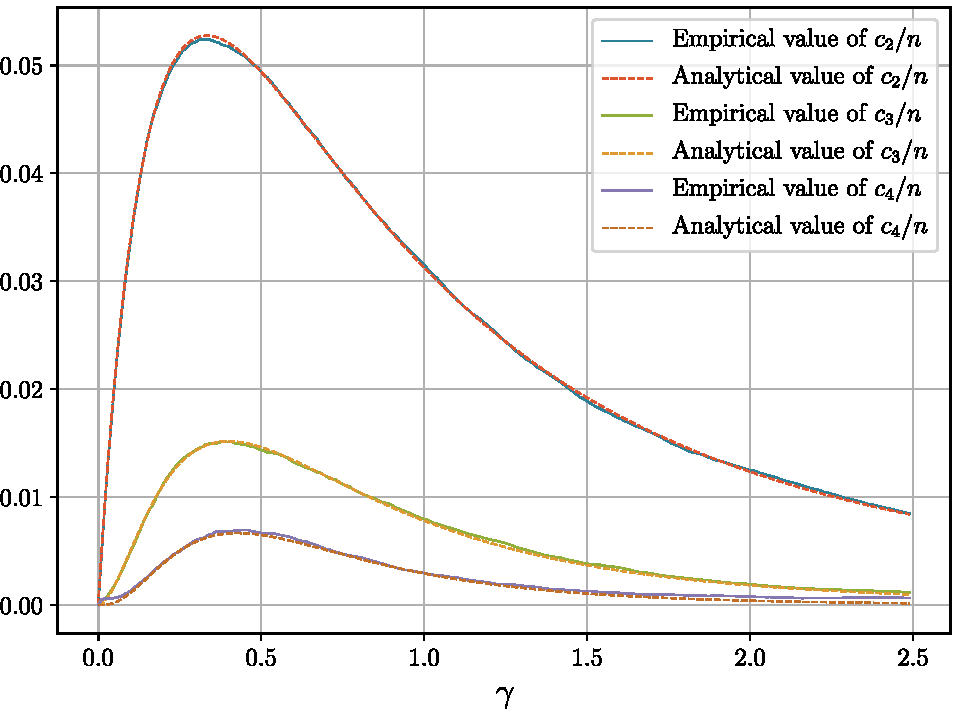
\includegraphics[width=0.9\linewidth]{img/cms_1.pdf}
    \caption{Сравнение эмпирических и теоретических результатов для нормированного количества циклов заданной длины}
    \label{cms}
\end{figure}

На рис.~\ref{cms} приведено сравнение результатов полученных эмпирическим и теоретическим способом.
Как мы видим, результаты достаточно хорошо совпадают и могут только незначительно отличаться при $\gamma \geq 1.5$, что связано с тем, что циклы меньшей длины могут получаться в результате распадения циклов большей длины.

Так как метод оценки основывается на статистиках $\frac b n$ и $\frac d n$ и их частном  $\frac b b$, построим подобный график и для них (рис.~\ref{d-b-n}).
\begin{figure}[h!]
    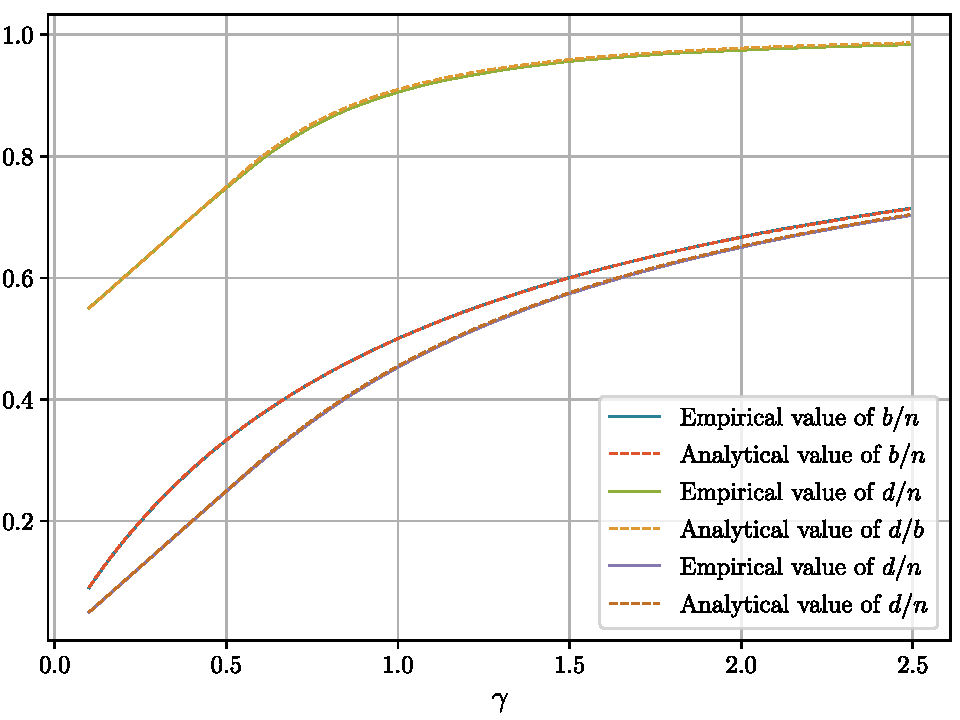
\includegraphics[width=0.9\linewidth]{img/d-b-n_1.pdf}
    \caption{Сравнение эмпирических и теоретических результатов для нормированного количества циклов заданной длины}
    \label{d-b-n}
\end{figure}
Как мы видим, в данном случае результаты совпадают ещё больше, и в некоторых моментах графики даже неразличимы.

\section{Сравнение с методом оценки Танье}
Для сравнения методов также будем использовать симулированные данные.
Для каждого $\gamma$ из отрезка $[0.3, 1)$ кратного $0.1$, попробуем предсказать, какое число шагов было сделано, и запишем соответствующую ошибку как $\frac {(k_e - k)} k$, где $k_e$ --- предсказанное число шагов, а $k$ --- реальное число шагов.
Для каждого соответствующего $\gamma$ было проведено 200 симуляций и построены соответствующие графики вида <<ящик с усами>>.
Как и ранее, <<ящик>> соответствует $50 \, \%$ результатов, а <<усы>>, в свою очередь, $90 \, \%$.

Важно отметить, что метод оценки не располагает информацией ни о реальном числе шагов, ни о количестве тривиальных циклов.
Вся информация, известная методу --- это количество циклов длин $l \geq 2$.

\begin{figure}[htb]
\centering
  \renewcommand{\thesubfigure}{а}
  \subfloat[Метод \textbf{Танье} на \textbf{больших} геномах]{%
    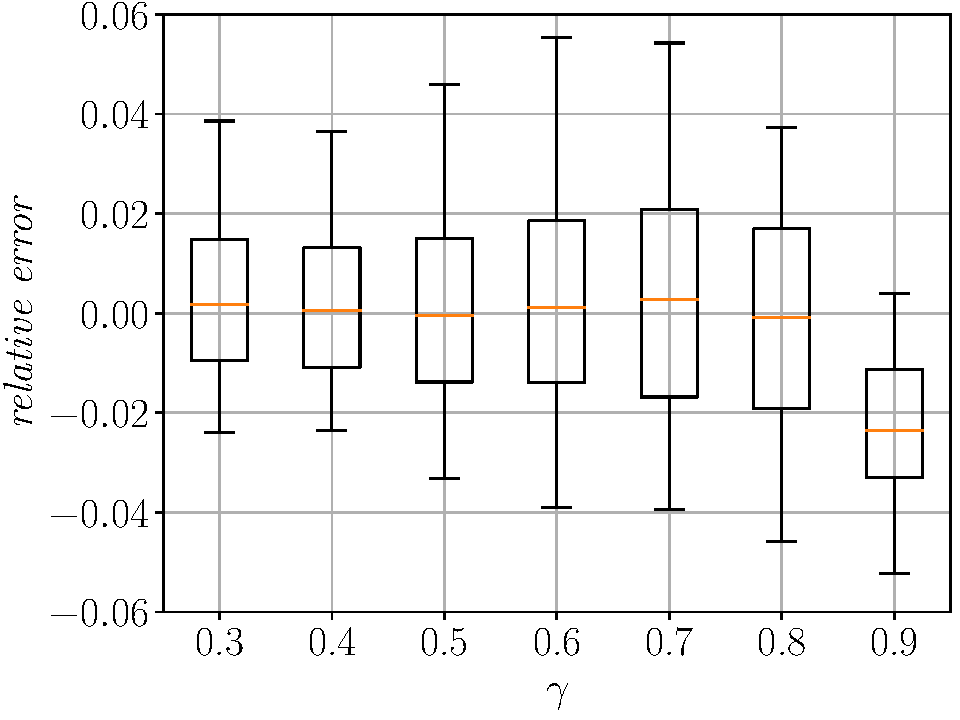
\includegraphics[width=.49\linewidth]{img/tan-est.pdf}}\hfill
  \renewcommand{\thesubfigure}{б}
  \subfloat[Метод \textbf{Танье} на \textbf{малых} геномах]{%
    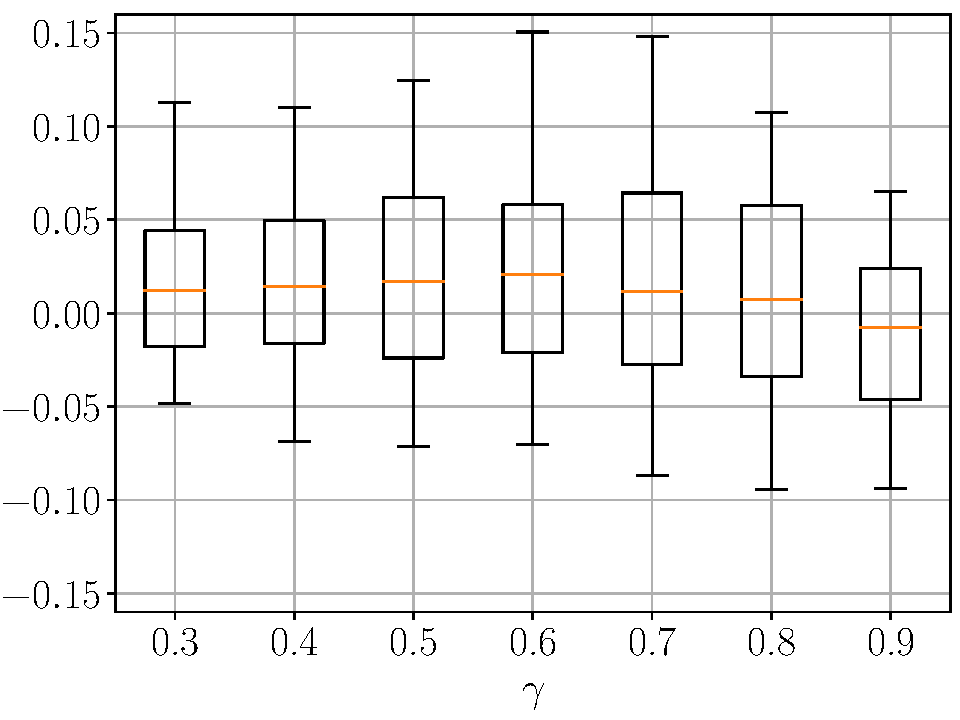
\includegraphics[width=.49\linewidth]{img/tan-est-small-n.pdf}} \\
  \renewcommand{\thesubfigure}{в}
  \subfloat[\textbf{Наш} метод  на \textbf{больших} геномах]{%
    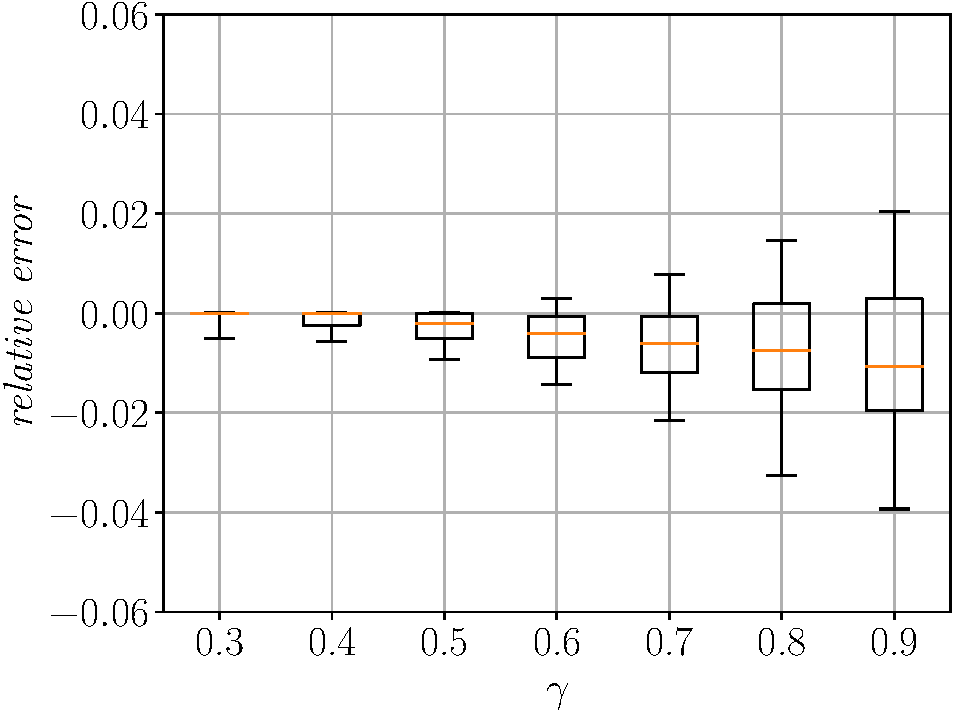
\includegraphics[width=.49\linewidth]{img/my-est.pdf}} \hfill
  \renewcommand{\thesubfigure}{г}
  \subfloat[\textbf{Наш} метод на \textbf{малых} геномах]{%
    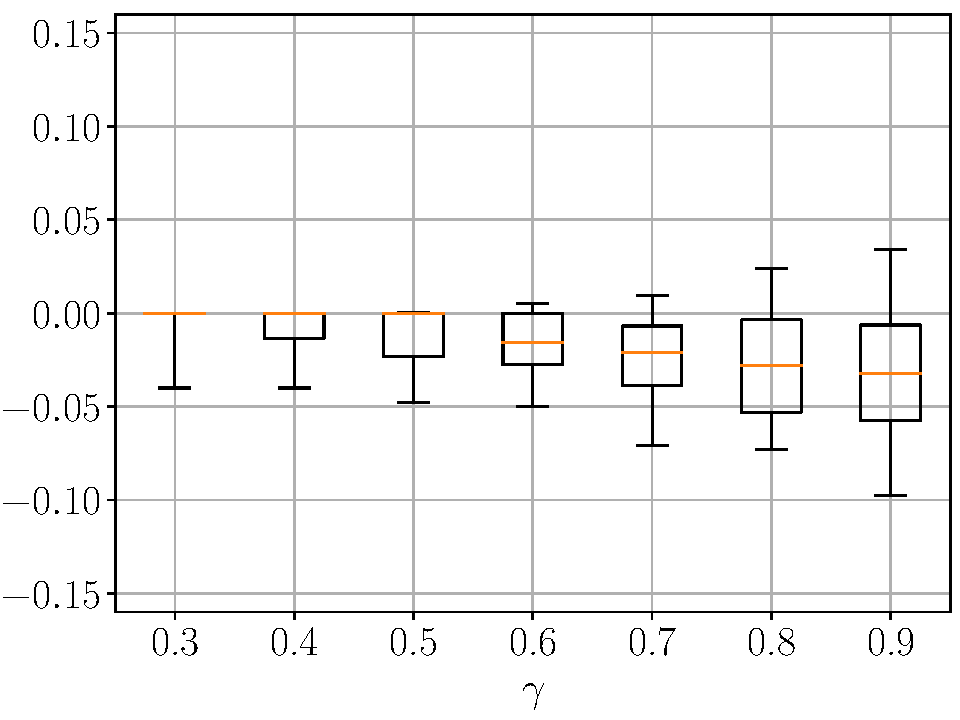
\includegraphics[width=.49\linewidth]{img/my-est-small-n.pdf}}
  \caption{Сравнение зависимости распределения относительной ошибки $\frac {k_e - k} k$ от $\gamma$ при оценке разными методами}
  \label{compare-methods}
\end{figure}


На рис.~\ref{compare-methods} показаны результаты работы разных методов для геномов разных размеров.
Для больших геномов $n$ находится в промежутке $[1000, 3000]$, для малых --- в промежутке $[200, 400]$.

Как мы видим, ошибка метода Танье для больших геномов находится в пределах $4 \, \%$ в $50 \, \%$ случаев, погрешность нашего же метода находится в пределах $2 \%$.
А в $90 \, \%$ случаев ошибка метода Танье находится в пределах $6 \, \%$, наш же метод ошибается не более, чем на $4 \, \%$.

Несмотря на то, что в нашей работе мы переходим к пределу по $n$, новый метод показывает лучшие результаты в сравнении с методом Танье.

Для малых геномов ошибка метода Танье находится в пределах $7 \, \%$ в $50 \, \%$ случаев, погрешность же нашего метода находится в пределах $6 \%$.
А в $90 \, \%$ случаев ошибка метода Танье находится в пределах $15 \, \%$, наш метод ошибается не более, чем на $10 \, \%$.

При больших $\gamma$ сравнить методы оценки не представляется возможным, так как метод Танье работает только при $k < \frac n 2$.

В главе 2 этой работы найдены теоретические оценки всех компонент, в то время как в работе \cite{fr-4} найдены оценки только для двух компонент, на которых построен метод оценивания. 
При этом одна из этих компонент $c_2$ имеет высокую дисперсию, что может негативно сказываться на точности оценки в случаях выбросов.

Оценки компонент, полученные в \cite{fr-4}, являются нелинейными, и для поиска оптимального решения используется решение системы двух нелинейных уравнений модифицированными градиентными методами.
Компонента $c_2$ немонотонна, что, однако, не влияет на результат.

В этой работе используются более простые и монотонные оценки, а для поиска корней - двоичный поиск.

Сравнение полученных оценок приведено в таблице ~\ref{comp-compare}:
\def\arraystretch{1.4}
\begin{table}[!h]
    \caption{Сравнение формул оценки необходимых компонент}
    \centering
    \begin{tabular}{|*{3}{c|}}\hline
            --              & Оценка Танье & Наша оценка \\\hline
            Оценка на $c_1$ &
            \(\displaystyle \sum_{l=0}^{\infty} \frac{(-2k)^l} {\prod_{u=0}^{l-1} (n+u)} \) &
            \(\displaystyle \frac {n^2} {2k + n} \) \\
        \hline
            Оценка на $c_2$ &
            \(\displaystyle k n^2 \sum_{l=0}^{\infty} \sum_{m=0}^{\infty} \frac{(-2(k-1))^{l+m}(l+1)(m+1)} {\prod_{u=0}^{l+m+1} (n+u)} \) &
            \(\displaystyle \frac {k n^4} {(2k + n)^4} \) \\
        \hline
    \end{tabular}
    \label{comp-compare}
\end{table}

Проведём сравнение реализаций данных методов.
Оба метода были реализованы на языке программирования \textit{Python 3}.
Так как метод Танье основывается на модифицированном градиентом спуске и имеет два нелинейных уравнения, была посчитана соответствующая матрица Якоби.
% тут можно написать формул для страху
Как было предложено в статье \cite{fr-4}, поиск оптимальных значений происходит с помощью метода \textit{optimize.root} из библиотеки \textit{scipy}.
Наш же метод использует метод двоичного поиска \textit{optimize.bisect} из той же библиотеки.

Измерения времени работы проведено на компьютере с процессором \textit{Core i5-5257U} и установленными \textit{Python} версии \textit{3.6.1} и библиотекой \textit{scipy} версии \textit{1.0.1}.

Важно отметить, что время работы ни одного из рассматриваемых методов оценки асимптотически никак не зависит от размера графа.
От размера графа зависит время, затрачиваемое на подсчёт необходимых компонент, и оно во всех случаях составляет $O(n)$, где $n$ --- число вершин в графе.
Подобная оценка достигается простым обходом в глубину.

Все измерения проводились на симулированных данных. Результаты приведены в таблице ~\ref{performance-compare}.
\begin{table}[!h]
    \caption{Сравнение работы методов}
    \centering
    \begin{tabular}{|*{3}{c|}}\hline
        -- & метод Танье & наш метод \\\hline
        \makecell{Среднее время работы \\ на малых геномах}       & 2.98 сек. & 0.00016 сек. \\\hline
        \makecell{Средний модуль ошибки \\ на малых геномах}      & 4.8 \%    & 2.1 \% \\\hline
        \makecell{Среднее время работы \\ на больших геномах}     & 3.02 сек. & 0.00017 сек. \\\hline
        \makecell{Средний модуль ошибки \\ на больших геномах}    & 1.99 \%   & 0.68 \% \\\hline
        Работает при $k \geq \frac n 2$                           & Нет       & Да \\\hline
        Реализация     & \makecell{Система уравнений и \\ модифицированный \\ градиентный спуск} & \makecell{Вещественный \\ двоичный поиск} \\\hline
    \end{tabular}
    \label{performance-compare}
\end{table}

\section{Применение метода к реальным данным}
\subsection{Семейство \emph{Rasacae}}

Для рассмотрения возьмем следующие геномы  видов из семейства \emph{Rosaceae}: \emph{Prunus} (слива), \emph{Fragaria} (клубника), \emph{Malus} (яблоко).
Геномные данные взяты из статьи \cite{real-data}.
Рассмотрим всевозможные пары этих геномов и запишем результаты в таблицу ~\ref{real-data-rasacae}.
\begin{table}[!h]
    \caption{Сравнения методов на реальных данных из семейства \emph{Rasacae}}
    \centering
    \begin{tabular}{|*{5}{c|}}\hline
        Пара геномов &  \makecell{Минимальное \\ расстояние}
                     & Наш метод
                     & Танье
                     & \makecell{Равновероятная \\ модель} \\\hline
        \emph{Prunus} --- \emph{Fragaria}    & 273 & 297 & 284 & 283     \\\hline
        \emph{Prunus} --- \emph{Malus}     & 261 & 263 & 258 & 261    \\\hline
        \emph{Fragaria} --- \emph{Malus} & 414 & 461 & 426 & 435   \\\hline
    \end{tabular}
    \label{real-data-rasacae}
\end{table}

Как можно увидеть из таблицы, истинное эволюционное растояние в рамках нашей модели может отличаться от минимального на $11 \, \%$ (это достигается в паре <<\emph{Prunus} --- \emph{Fragaria}>>).
В то время как классический подход (равновероятная модель) к оценке истинного расстояния показывает разницы всего в $5 \, \%$.
Заметим, что разница такого порядка является статистически значимой; вероятность того, что она  является результатом погрешности измерений не превосходит $1 \, \%$.

Аналогичная ситуация происходит на паре <<\emph{Prunus} --- \emph{Fragaria}>>, в рамках нашей модели разница с минимальным расстоянием достигает $8.7 \, \%$, а в рамках равновероятной модели эта цифра составляет $4 \, \%$.

Пара <<\emph{Prunus} --- \emph{Malus}>> в нашей модели находится немного за границей парсимонии, а в рамках модели равновероятной перед ней.
Поэтому различие в минимальном и истинном расстоянии мы видим только в рамках нашей модели.

Метод Танье на предложенных данных показывает себя чуть хуже.
Результаты его работы примерно равны результатам оценщика классического.
За исключением того факта, что в паре <<\emph{Prunus} --- \emph{Malus}>> он показал результат меньший, чем минимальное расстояние.
Вероятно это связно с тем, что произошёл выброс по компоненте $c_2$.

\subsection{Класс \emph{Mammalian}}
Для следующего рассмотрения возьмем геномы  видов из класса \emph{Mammalian} (млекопитающие): \emph{Rat} (крыса), \emph{Chimpanzee} (шимпанзе), \emph{Dog} (собака), \emph{Mouse} (мышь), \emph{Macaque} (макака), \emph{Human} (человек).
Рассмотрим всевозможные пары этих геномов и запишем результаты в таблицу ~\ref{real-data-mammalian}.
\begin{table}[!h]
    \caption{Сравнения методов на реальных данных из класса \emph{Mammalian}}
    \centering
    \begin{tabular}{|*{5}{c|}}\hline
        Пара геномов &  \makecell{Минимальное \\ расстояние}
                     & Наш метод
                     & Танье
                     & \makecell{Равновер. \\ модель} \\\hline
                    \emph{Chimpanzee} --- \emph{Dog}    & 312 & 312 & 287 & 312     \\\hline
                    \emph{Chimpanzee} --- \emph{Human}    & 22 & 22 & 22 & 22     \\\hline
                    \emph{Chimpanzee} --- \emph{Mouse}    & 420 & 426 & 379 & 420     \\\hline
                    \emph{Chimpanzee} --- \emph{Macaque}    & 115 & 115 & 118 & 115     \\\hline
                    \emph{Chimpanzee} --- \emph{Rat}    & 724 & 724 & 703 & 724     \\\hline
                    \emph{Dog} --- \emph{Human}    & 304 & 304 & 278 & 304     \\\hline
                    \emph{Dog} --- \emph{Mouse}    & 450 & 456 & 409 & 450     \\\hline
                    \emph{Dog} --- \emph{Macaque}    & 301 & 301 & 275 & 301     \\\hline
                    \emph{Dog} --- \emph{Rat}    & 756 & 756 & 733 & 756     \\\hline
                    \emph{Human} --- \emph{Mouse}    & 408 & 414 & 370 & 408     \\\hline
                    \emph{Human} --- \emph{Macaque}    & 106 & 106 & 109 & 106     \\\hline
                    \emph{Human} --- \emph{Rat}    & 714 & 714 & 694 & 714     \\\hline
                    \emph{Mouse} --- \emph{Macaque}    & 407 & 407 & 367 & 407     \\\hline
                    \emph{Mouse} --- \emph{Rat}    & 454 & 454 & 464 & 454     \\\hline
                    \emph{Macaque} --- \emph{Rat}    & 706 & 706 & 690 & 706     \\\hline
    \end{tabular}
    \label{real-data-mammalian}
\end{table}

Как можно увидеть из таблицы, в рамках модели с равновероятными поломками рёбер, все пары геномов находятся на стадии парсимонии. 
То есть оценка на истинное эволюционное расстояние совпадает с минимальным расстоянием.

В рамках нашей модели три пары геномов находятся за границей парсимонии и отличаются примерно на $1.5 \, \%$. 
Этими парами являются: \emph{Chimpanzee} --- \emph{Mouse}, \emph{Dog} --- \emph{Mouse} и \emph{Human} --- \emph{Mouse}.
Это говорит о том, что \emph{Mouse} более удалена от остальных видов из класса \emph{Mammalian} (млекопитающие) взятого набора.

Метод Танье на рассматриваемых видах показывает себя неудовлетворительно.
В $11$ парах из $15$ (\emph{Chimpanzee} --- \emph{Dog}, \emph{Chimpanzee} --- \emph{Mouse}, \emph{Chimpanzee} --- \emph{Rat}, \emph{Dog} --- \emph{Human}, \emph{Dog} --- \emph{Mouse}, \emph{Dog} --- \emph{Macaque}, \emph{Dog} --- \emph{Rat}, \emph{Human} --- \emph{Mouse}, \emph{Human} --- \emph{Rat}, \emph{Mouse} --- \emph{Macaque}, \emph{Macaque} --- \emph{Rat}) оценка на истинное расстояние меньше, чем минимальное расстояние. 
Причём, подобная ошибка достигает $9.8 \, \%$ в случае пары \emph{Mouse} --- \emph{Macaque} и некоторых других, что показывает неприменимость метода Танье к данным видам. 
Данная ошибка, вероятнее всего, связана с выбросом по компоненте $c_2$.

\subsection{Род \emph{Shigella}}
Для последнего рассмотрения возьмем геномы  видов из класса \emph{Shigella}: \emph{Shigella sonnei Ss046}, \emph{Shigella boydii Sb227}, \emph{Shigella boydii CDC 3083 94}, \emph{Shigella flexneri 2a}, \emph{Shigella flexneri 5 8401}, \emph{Shigella flexneri 2a 2457T}.
Рассмотрим всевозможные пары этих геномов и запишем результаты в таблицу ~\ref{real-data-shigella}.
\begin{table}[!h]
    \caption{Сравнения методов на реальных данных из рода \emph{Shigella}}
    \centering
    \begin{tabular}{|*{5}{c|}}\hline
        Пара геномов &  \makecell{Мин. \\ расст.}
                     & Наш метод
                     & Танье
                     & \makecell{Равновер. \\ модель} \\\hline
                    \makecell{ \emph{S. s. Ss046} --- \emph{S. b. Sb227} }    & 32 & 32 & 31 & 32     \\\hline
                    \makecell{ \emph{S. s. Ss046} --- \emph{S. b. CDC 3083 94} }    & 44 & 46 & 47 & 44     \\\hline
                    \makecell{ \emph{S. s. Ss046} --- \emph{S. f. 2a} }    & 43 & 45 & 46 & 43     \\\hline
                    \makecell{ \emph{S. s. Ss046} --- \emph{S. f. 5 8401} }    & 40 & 40 & 40 & 40     \\\hline
                    \makecell{ \emph{S. s. Ss046} --- \emph{S.f. 2a 2457T} }    & 35 & 35 & 40 & 35     \\\hline
                    \makecell{ \emph{S. b. Sb227} --- \emph{S. b. CDC 3083 94} }    & 42 & 42 & 45 & 42     \\\hline
                    \makecell{ \emph{S. b. Sb227} --- \emph{S. f. 2a} }    & 45 & 45 & 46 & 45     \\\hline
                    \makecell{ \emph{S. b. Sb227} --- \emph{S. f. 5 8401} }    & 40 & 40 & 40 & 40     \\\hline
                    \makecell{ \emph{S. b. Sb227} --- \emph{S.f. 2a 2457T} }    & 35 & 35 & 34 & 35     \\\hline
                    \makecell{ \emph{S. b. CDC 3083 94} --- \emph{S. f. 2a} }    & 9 & 9 & 9 & 9     \\\hline
                    \makecell{ \emph{S. b. CDC 3083 94} --- \emph{S. f. 5 8401} }    & 14 & 14 & 15 & 14     \\\hline
                    \makecell{ \emph{S. b. CDC 3083 94} --- \emph{S.f. 2a 2457T} }    & 28 & 28 & 29 & 28     \\\hline
                    \makecell{ \emph{S. f. 2a} --- \emph{S. f. 5 8401} }    & 11 & 11 & 12 & 11     \\\hline
                    \makecell{ \emph{S. f. 2a} --- \emph{S.f. 2a 2457T} }    & 29 & 29 & 30 & 29     \\\hline
                    \makecell{ \emph{S. f. 5 8401} --- \emph{S.f. 2a 2457T} }    & 24 & 24 & 25 & 24     \\\hline
    \end{tabular}
    \label{real-data-shigella}
\end{table}

Как можно увидеть из таблицы для видов из рода \emph{Shigella}, в рамках модели с равновероятными поломками рёбер все пары геномов опять же находятся на стадии парсимонии. 
То есть минимальное расстояние совпадает с оценкой на истинное эволюционное расстояние.

При этом в рамках нашего метода $2$ пары (\emph{S. s. Ss046} --- \emph{S. b. CDC 3083 94}, \emph{S. s. Ss046} --- \emph{S. f. 2a}) выходят за границу парсимонии.
Оценка на расстояние отличается от минимального отличается всего на $2$ шага, но эти $2$ шага дают отличие на $4.5 \, \%$, что является заметным различием.

Метод Танье на видах рода \emph{Shigella} показывает себя лучше, чем на предыдущих.
Только в случае одной пары оценка на истинное расстояние оказывается меньше, чем  минимальное расстояние(\emph{S. b. Sb227} --- \emph{S.f. 2a 2457T}).
На тех же двух парах, которые выходили за границу парсимониив в нашем методе, также достигается выход за границу. 
Но выход за подобную границу достигается и на многих других парах:
\emph{S. s. Ss046} --- \emph{S.f. 2a 2457T},
\emph{S. b. Sb227} --- \emph{S. b. CDC 3083 94},
\emph{S. b. Sb227} --- \emph{S. f. 2a},
\emph{S. b. CDC 3083 94} --- \emph{S. f. 5 8401},
\emph{S. b. CDC 3083 94} --- \emph{S.f. 2a 2457T},
\emph{S. f. 2a} --- \emph{S. f. 5 8401},
\emph{S. f. 2a} --- \emph{S.f. 2a 2457T},
\emph{S. f. 5 8401} --- \emph{S.f. 2a 2457T}.

\subsection{Оценка производительности на реальных данных}
Несмотря на то, что скорость работы метода оценки не зависит асимптотически от размера генома, для полноты картины проведём оценку на скорость работы методов на реальных данных.
Для этого замерим среднее время работы каждого метода на всевозможных парах реальных данных рассмотренных выше, включая время на преобразование генома в граф точек и вычисление необходимых компонент. 
Результаты приведены в таблице ~\ref{real-data-time}.
\begin{table}[!h]
    \caption{Среднее время работы методов}
    \centering
    \begin{tabular}{|*{4}{c|}}\hline
        Набор геномов & Наш метод
                      & Танье
                      & \makecell{Равновероятная \\ модель} \\\hline
        Семейство \emph{Rasacae} & 0.012 сек. & 3.13 сек. & 0.015 сек. \\\hline
        Класс \emph{Mammalian}   & 0.027 сек. & 3.55 сек. & 0.037 сек. \\\hline
        Род \emph{Shigella}      & 0.004 сек. & 2.93 сек. & 0.008 сек. \\\hline
    \end{tabular}
    \label{real-data-time}
\end{table}

\chapterconclusion
В главе 3 был проведен эмпирический анализ модели и сравнение с теоретическими результатами.
Также было проведено сравнение нового метода оценки с методом, предложенным в \cite{fr-4}. Это сравнение показало более высокие точность, эффективность и применимость указанного метода.

Разные методы оценки расстояния были применены к реальным данным.
Основываясь на этих данных показано, что истинное эволюционное расстояние может отличаться от минимального до $11 \, \%$.
%!!! это Вы  как-то скромно, мы  же не все на свете пары организмов перебрали.
%!!! но оставьте так
И наконец, ввиду измененной границы парсимонии, показано, что в рамках рассматриваемой модели парсимония может не достигаться там, где она достигалась ранее.